\chapter{A Modular Region and Text Line Layout Analysis System}
\chaptermark{Region and Text Line Layout Analysis}
\thispagestyle{empty}
\vfill
This chapter has been published as \fullcite{KiesslingICFHR2020}. The layout
analysis method presented herein corresponds to the current implementation in
the Kraken engine apart from slight changes in line end marker shapes and
postprocessing.
\label{ch:icfhr}
\newpage

\section*{Abstract}
High quality document layout analysis is fundamental to the accurate processing
of handwritten textual material, on both the level of individual lines and
higher order zones demarking textual and non-textual content. We present an
artificial neural network based approach to prediction of either that is
implemented as part of a libre optical character recognition package and highly
reconfigurable for a variety of tasks. Experiments on different openly
available datasets show competitive results to state-of-the-art methods.

\section{Introduction}

Over the last decades tremendous amounts of historical handwritten documents
have been digitized by archives, libraries, and other institutions engaging in
the preservation of cultural heritage. Nevertheless the vast volume of scanned
images, often with lack of metadata, results in the majority of this material
being inaccessible in any meaningful way to scholars and the wider public.
Optical Character Recognition\footnote{As methods have converged considerably
we do not distinguish between recognition of printed (OCR) and handwritten text
(HTR)} and Keyword Spotting aim to be technical solutions to the exploitation
of large amounts of scanned textual data. 

Current OCR systems operate largely on \emph{line}-level data, i.e. the module
in the OCR pipeline performing conversion into text does so one line image at a
time. Therefore, a prior method is needed to extract these line images from
whole document images. In addition, many documents require higher level
understanding of how lines relate to each other for meaningful interaction. The
usual way these higher level relations are modelled is through zoning, i.e.
splitting a page into regions such as main text, marginalia, headings,
illustrations, etc. Importantly, the nature of those regions can vary
considerably between applications and material; they can often overlap, lines
might extend across them or not be in any region at all. Consequently, text
line extraction and region detection are arguably the most important part of an
OCR system apart from the actual text recognizer.

As such, robust and accurate historical and handwritten document image analysis
remains an open issue despite the recent advances facilitated by deep learning
methods. Highly curved lines, variable orientation, interlinear notes, and
multiple texts on the same page remain challenging to even state of the art
layout analysis systems. Further, cultural bias in the conception of methods
and data models continues to be a persistent problem: \cite{kiessling2019badam}
shows the large amount of adaptation necessary to apply a seemingly
script-neutral line model to Arabic manuscripts.

For our purposes we consider layout analysis along two principal axes. The
\emph{geometric axis} deals with the location, shape, and relations of found
entitites, e.g. the by now obsolete character segmentation, text line
extraction, and region detection. Text line extraction refers to the locating
of individual text lines in the document images. In most modern LA systems text
lines are the smallest unit of output, albeit for specialized tasks like scene
text recognition subdivisions into words is also widespread. Region detection
aims to find higher level, almost exclusively structural, zones, both textual
and not, in document images. 

The \emph{semantic axis} concerns itself with the functional nature of detected
entities, such as titles, illustrations, apparatus criticus, \dots. While not
strictly necessary for most applications and often neglected outside of tools
tailored for specific input data, enriching with semantic information can both
boost raw metrics through allowing better incorporation of domain knowledge and
aid in human understanding by improving output structuring, such as suppressing
certain ancillary textual components.

Of note is that the focus of most methods is limited to a single or a subset of
the tasks and axes. For example, no method could be found that allows semantic
classification of both region and text line detection output simultaneously. In
contrast, our method admits geometric and semantic classification on both text
lines and regions while not requiring either.

Our method is implemented as part of a free OCR engine\footnote{\texttt{http://kraken.re}}
which exposes the full customizability of the method's layout analysis features
to end users.  Hence, we are referring to the system as modular; it is possible
to perform a wide range of tasks, ranging from simple text line extraction to
highly specialized analysis like writing surface defect detection in a unified
software package.

\subsection{Related work}

As a well established task in computer vision research a number of
comprehensive surveys of document layout analysis exist
\cite{binmakhashen2019document, eskenazi:hal-01388088, nagy2000twenty}. 

\subsection{Text line extraction}

\begin{figure*}[ht]
        \centering
        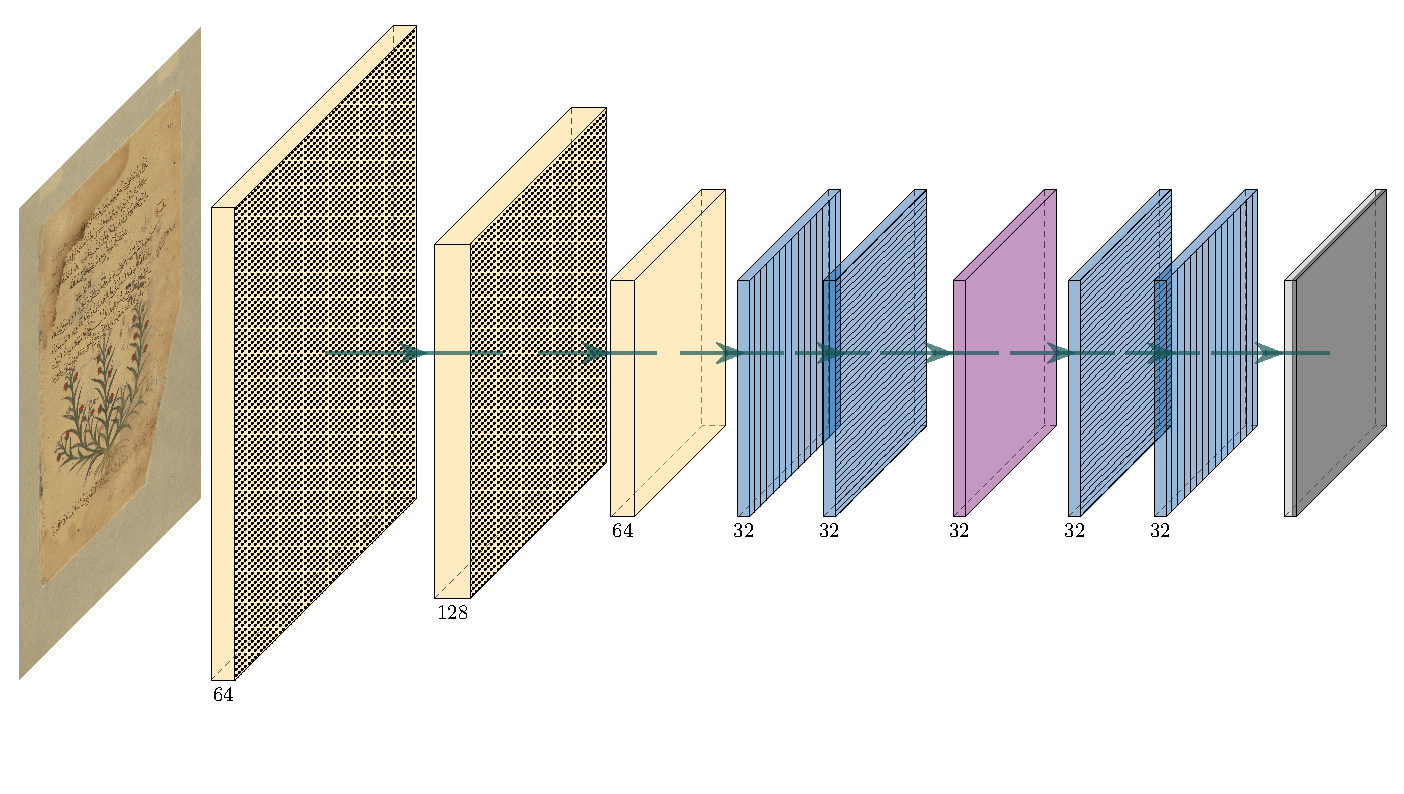
\includegraphics[width=\textwidth]{rblla}
	\caption{Architecture of the pixel labelling network. Group
	normalization layers are omitted. (salmon: 3x3 convolutional layers,
	dotting indicates dilation by 2x2; purple: 1x1 convolution, blue:
	bidirectional LSTM blocks, striping indicates row/column time axis;
	grey: 1x1 convolution with $\norm{\tau}$ filters + sigmoid)}
	\label{fig:rblla}
\end{figure*}

The capabilities of text line extraction methods in the literature is to some
extent driven by existing datasets. A variety of formulations for line
extraction can be found in published datasets. These range from polygons
\cite{fischer2011transcription,simistira2016diva,clausner2018icfhr}, to
sub-word bounding boxes \cite{kassis2017vml}, down to explicit pixel labeling
\cite{gatos2010icfhr}. Some others such as
\cite{antonacopoulos2015icdar2015,antonacopoulos2011historical} also include
extensive metadata like reading order, text order, or full transcriptions. A
recent model \cite{diem2017cbad} reduces text line detection to the extraction
of baselines, i.e. imaginary polylines upon which the text rests or hangs from.
These polylines in combination with a bounding polygon can be ingested by
line-based text recognizers with minimal adaptation while at the same time
requiring only modest effort for manual annotation, encouraging the creation of
substantial training datasets for machine learning based methods.

The methods employed for text line extraction are just as varied as the the
data models employed. \cite{ouwayed2012general, borse2014language} use
connected components combined with filtering to perform pixel labeling. A
common paradigm utilizes projection profiles in one way or another such as
\cite{diem2013text} for bounding box extraction, \cite{arvanitopoulos2014seam,
saabni2014text} in combination with seamcarving for polygonal output, or
RNN-based artificial projection profile generation for in-paragraph line
splitting in \cite{moysset2015paragraph}. A common drawback of the previously
mentioned methods is that they operate on binarized input images which can be
difficult to obtain for degraded historical material.
\cite{garz2012binarization, ahn2017textline, gruuening2017robust}
bypass this requirement through clustering of superpixels that can be obtained
directly from color or grayscale image data to calculate polygons and baselines
respectively. A number of deep learning based schemes have been proposed as
well: \cite{mechi2019text, quiros2018multi, oliveira2018dhsegment}
apply variants of the U-Net architecture for semantic segmentation.


\subsection{Region detection}

Region detection is almost always performed across both the geometric and
semantic axis although they vary in the variety of zone labels they can
yield. The most basic methods such as \cite{baechler2011multi,
chen2014page} only distinguish between text and non-text regions while
\cite{dejean2019versatile} can in principle be extended to all textual regions
determinable solely by layout relations, and \cite{soullard2020multi,
quiros2018multi, oliveira2018dhsegment, kaddas2018deep} are able to distinguish
arbitrary, non-overlapping regions with appropriate training data.

Like for text line extraction \cite{soullard2020multi,quiros2018multi,
oliveira2018dhsegment} variants of convolutional
encoder-decoder networks are popular albeit pixel classifiers on handcrafted
features \cite{chen2014page, baechler2011multi} exist.
\cite{dejean2019versatile} performs clustering of text lines with convolutional
conjugate graph networks.  Definite clause grammars on a feature vocabulary as
part of a user-driven interactive segmentation system are shown in
\cite{lemaitre2008multiresolution}.

\begin{wrapfigure}{o}{0.5\textwidth}
	\centering
	\begin{subfigure}{0.48\textwidth}
		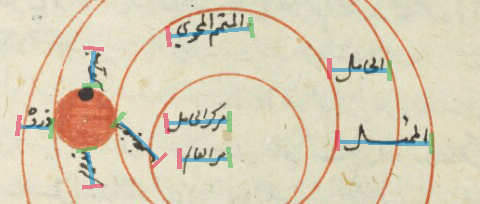
\includegraphics[width=\textwidth]{overlay_crop.png}
		\caption{Ground truth overlay for a page with different line
		orientations (blue: baseline class, red: start\_sep auxiliary
		class, green: end\_sep auxiliary class)}
		\label{fig:overlay}
	\end{subfigure}
	\vskip\baselineskip

	\begin{subfigure}{0.48\textwidth}
		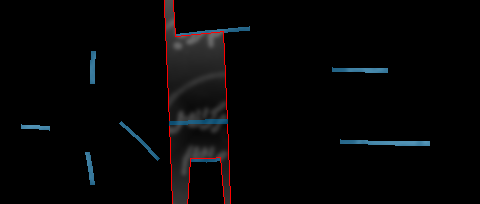
\includegraphics[width=\textwidth]{roi_crop.png}
		\caption{Region of Interests of the distance biased energy map for a sample line of the same image. (red: border of RoIs, blue: baselines)}
		\label{fig:roi}
	\end{subfigure}
	\vskip\baselineskip

	\begin{subfigure}{0.48\textwidth}
		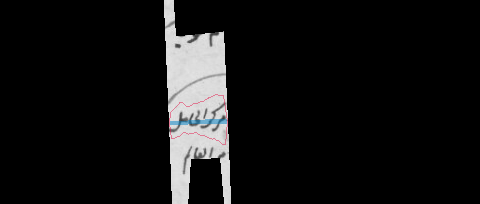
\includegraphics[width=\textwidth]{seam_crop.png}
		\caption{Computed seam/bounding polygon on the masked input image crop. (red: combined upper and lower half-seams, blue: baselines)}
		\label{fig:seam}
	\end{subfigure}
	\caption[Examples of the data model and intermediate representations
		 for a page from the BADAM dataset]{Examples of the data model and intermediate representations
		 for a page from the
		 BADAM~\protect\cite{kiessling2019badam} dataset}
\end{wrapfigure}
\section{Method}


This section describes the proposed method for joint text line and region
layout analysis. Our method can be divided into three main stages: multi-label
pixel classification, baseline extraction and polygonization, and region
extraction.

The first stage comprises of an Artifical Neural Network which outputs the
probability of one or more classes (baselines, regions, and auxiliary classes)
being present for each pixel of the input image. The second stage consists of
the postprocessing extracting baselines from the auxiliary and baseline classes
heatmaps, followed by a seam-carving step incorporating the original image to
compute the bounding polygons required for inclusion of our method in a fully
functional OCR pipeline.  The final step extracts the regions from their
respective class heatmaps through a contour finding algorithm. Notably,
baselines are not restricted to regions, i.e. they can occur outside of regions
and cross region boundaries. 

\subsection{R-BLLA - Architecture}

The overall pixel labeling network neural network is described in figure~\ref{fig:rblla}. Instead of conventional semantic segmentation encoder-decoder
networks whose output is at the same scale as the input, our architecture
decodes the learned representations at the downsampled scale of the last layer
as the spatial information of regions and baselines can be recovered with
sufficient accuracy at this reduced resolution. This architecture roughly
halves the memory requirements in comparison to an equivalent U-Net with a
Resnet-50 backbone.

Our network is composed of a convolutional feature extractor, utilizing atrous
convolutions ($3 \times 3$ kernel size with $2 \times 2$ dilation, ReLU
activation) to increase receptive field without increasing filter size or a
more memory intensive deeper decoding network. This convolutional stack is
followed by consecutive unidimensional LSTM layers as proposed for the ReNet
architecture \cite{visin2015renet}. In this configuration the feature maps from
the previous layers are swept by a bidirectional 1D LSTM layer in one direction
(vertical or horizontal), followed by a second sweep over the output by a LSTM
layer in the other direction, attaining similar performance to more complex
multidimensional RNNs. The final decoding layer is a $1\times 1$ convolution
with $\norm{\tau}$ filters and a sigmoid activation function that results in
per class probability maps.  Regularization is performed with group
normalization ($G=32$) \cite{DBLP:journals/corr/abs-1803-08494} after each
convolutional layer.

The output of the network is a stack of probability maps $\hat{y} \in
\mathbb{R}^{w/n \times h/n \times \norm{\tau}}$ for an input image $I \in
\mathbb{R}^{w\times h\times c}$ with height $h$, width $w$, $c$ channels, a
downsampling factor $n$, and $\norm{\tau}$ different classes $\{\text{start\_sep},
\text{end\_sep}, bl_0, \dots, bl_k, reg_0, \dots, reg_l\}$ for $k$ and $l$ different
baseline and region types. The special classes start\_sep and end\_sep are
placed at the beginning and end of each baseline respectively and serve two
purposes. First, by explicitly encoding line bounds at locations where lines
can be minimally separated such as multi-column texts we avoid inadvertent
baseline merging during postprocessing. Second, introducing separate indicator
classes for the beginning and end of a line allows the system to determine the
orientation of lines. These auxiliary classes are shared across all possible
baseline classes $\{bl_0, \dots, bl_k\}$. As our method is intended to work
with most scripts, including multi-script documents, the beginning and end of
each line is not determined by the reading direction of the script. Instead we
treat all scripts as canonically left-to-right, i.e when following the baseline
from the start marker the upper part of the text line is always on the
left-hand side (figure~\ref{fig:overlay}). This scheme makes processing of
arbitrarily oriented lines and mixed script pages with different reading
direction without additional domain knowledge possible. The generated ground
truth for the baselines classes are simple polylines drawn with a width.
Regions are encoded
as filled polygons. Thus the ground truth $y$ is a multi-hot encoded tensor.

\subsection{Training}



The network is trained in a supervised manner with binary cross-entropy loss
$L(y, \hat{y}) = \frac{1}{N}\sum^N_{i=0}(y\cdot \log(\hat{y}_i)+(1-y)\cdot
\log(1-\hat{y}_i))$. We adopt the Adam optimizer with moderate weight decay
($\alpha = 20^{-5}, \beta_1 = 0.9, \beta_2 = 0.999, w = 10^{-6}$). Input data
are whole RGB color images scaled to a height of 1200 pixels.

In line with conventional practice, data augmentation is applied to the
training set. With a probability of $0.5$ a set of randomly parametrized
transformations such as rotation, flipping, blurring, shifting, elastic
transformations and hue changes are applied to each image \cite{info11020125}.

We train for a fixed number of epochs, per default $50$.

\subsection{Baseline vectorization }

Baseline vectorization refers to the extraction of baselines from the
probability map output of the model. This task consists of multiple substeps:
superpixel calculation, triangulation filtering, and interpolation.

As the process is identical for each baseline type we define the output of the
neural network for an arbitrary baseline type $H = \hat{y}_{:,:,n}, n \in
\{bl_0, \dots, bl_k\}$. $P = \hat{y}_{:,:,\text{start\_sep}}, Q =
\hat{y}_{:,:,\text{end\_sep}}$.  Further we define a combined separator map $C = P + Q$.

In a first step we reduce the number of pixels to be considered for baseline
clustering through calculating a subset $T$ of all image pixels. Elements of
this subset are called superpixels (SPs). Determining SPs is largely identical
to the algorithm proposed in \cite{gruning2019two}. For an arbitrary
probability map $H$ the map is binarized with a threshold $0.2$ producing $H_b$
and skeletonized with a medial axis transformation that also returns a distance
transform of $H_b$, resulting in the skeleton $H_s$ and the  average
diameter $d_{cc}$ of each uneroded baseline. All foreground pixels in $H_s$ are
projected onto $H$ and sorted in descending order by their probability ($S$).
$T$ is iteratively filled by removing elements from $T$ as long as their
distance exceed a minimum ($d_{min} = 10$) from all other pixels in $S$.

\begin{algorithm}[H]
\caption{Triangulation filter}
\label{alg:dt_filter}
\begin{algorithmic}[1]
	\renewcommand{\algorithmicrequire}{\textbf{Input:}}
	\REQUIRE $DT(T), H, C$ 
	\STATE $E = \emptyset$
	\FOR {$e_{p, q} \in DT(T)$}
		\IF {$\mu(H, e_{p,q}) \geq 0.4 \land \sigma^2(H, e_{p,q}) \leq 0.05$}
			\IF {$\mu(C, e_{p,q}) \leq 0.125 \land \max(C, e_{p,q}) \leq 0.25$}
			\STATE {$E \leftarrow e_{p,q}$}
			\ENDIF
		\ENDIF 
	\ENDFOR
	\RETURN $E$
\end{algorithmic}
\end{algorithm}

The following step of the vectorization algorithm filters the Delaunay
triangulation $DT(T)$ of $T$ to subdivide it into a set of baseline clusters.
An edge between two SPs $p, q \in DT(T)$ is denoted by $e_{p, q}$. As a
prerequisite of the filtering algorithm we also define a number of edge
metrics. Given the discrete line coordinates produced by a line drawing method
$l(e_{p, q})$ between the SPs $p, q$ we define for an arbitrary map $I \in \{H,
P, Q\}$:

\begin{eqnarray*}
	\mu(I, e_{p, q}) &= \frac{1}{\norm{p - q}_2}\sum I[l(e_{p, q})]\\
	\sigma^2(I, e_{p, q}) &= \frac{1}{\norm{p - q}_2}\sum (I[l(e_{p, q})] - \mu(I, e_{p, q}))^2\\
	\max(I, e_{p, q}) &= \max(I[l(e_{p, q})])
\end{eqnarray*}

The output of the filtering algorithm Alg. \ref{alg:dt_filter} is a set of
edges $E$ defining a euclidean distance-weighted graph graph $G_E = G(V, E, w)$
where $V=\bigcup \{p, q\}, \forall e_{p,q} \in E, w(e_{p, q})= \norm{p - q}_2,
$ with a set of components $C^{G_E}$. Each component $C^{G_E}_n$ is treated as
a separate baseline cluster. The remaining task is to create a directed
polyline representation of each cluster. For each cluster we calculate the
pairwise distances of all vertices and select the two most distant nodes $a, b$
as the extrema of the baseline. The polyline approximation of each cluster is
the shortest path $\gamma_{a, b}$ between the extrema in $C^{G_E}_n$. A slight
correction of the line coordinates is necessary to compensate for the erosion
incurred through the skeletonization prior to superpixel selection. The
adjusted polyline path $\gamma_{a', b'}$ of $\gamma_{a, b}$ is obtained by
elongating the initial and last edges by $d_{cc}$.

Due to the unknown orientation of each line we inspect each line end's affinity
to the difference between the separator classes. As the separators are placed
beyond the end of the line, the values of the separator maps at those points
are commonly close to $0$. By preprocessing $P, Q$ with a maximum filter of
size $2 \cdot d_{min}$ resulting in maps $P', Q'$ containing sufficiently
dilated separators the correct line orientation is such that:

\begin{equation*}
	L(\gamma_{a', b'}, P', Q') = 
	\begin{cases}
		\gamma_{a', b'} &\text{if}
				\!\begin{aligned}[t]
					(P'-Q')_p &> 0.2 \land \\
					(Q'-P')_q &> 0.2
				\end{aligned}\\
		rev(\gamma_{a', b'}) & \text{if}
				\!\begin{aligned}[t]
					(P'-Q')_p &> 0.2 \land \\
					(Q'-P')_q &> 0.2
				\end{aligned}
	\end{cases}
\end{equation*}

otherwise 

\begin{equation*}
	L(\gamma_{a', b'}, P', Q') = 
	\begin{cases}
		\gamma_{a', b'} & a'_x \leq b'_x\\
		rev(\gamma_{a', b'}) & a'_x > b'_x
	\end{cases}
\end{equation*}

The final baselines for each baseline class is the set of all paths $\Gamma_m =
\{\gamma_1, \dots, \gamma_o\}, m \in \{bl_0, \dots, bl_k\}, o \in \mathbb{N}$ determined as above.

\subsection{Polygonization}

For recognition by an HTR engine the vectorized baselines have to be
supplemented by full polygons. A baseline with polygon can then rectified to
produce a normalized line image with suppression of non-line content by
projection onto a straight baseline through a piecewise affine transformation,
allowing recognition of even highly curved lines by text recognition models.

Our polygonization algorithm consists of a line-wise seam carving
\cite{avidan2007seam} biased by distance from the baseline. The initial energy
map is the derivative of the smoothed grayscale input image $I^\sigma$:

\begin{equation*}
	E(I^\sigma) = \left\vert\frac{\partial(I^\sigma)}{\partial x} + \frac{\partial(I^\sigma)}{\partial(y)}\right\vert
\end{equation*}

The primary purpose of the smoothing is to prevent the seam from crossing below
disconnected line components such as diacritics and tonal marks. A gaussian
filter with $\sigma = 2.5$ is sufficient for this purpose. Our implementation
estimates the gradient with the Sobel operator.

Let $\{\Gamma_0, \dots, \Gamma_n, \dots, \Gamma_m\}, 0 < n < m, m \in \{bl_0,
\dots, bl_k\}$ be the baselines of all classes and $\gamma \in \Gamma_n$ be an
arbitrary baseline. To calculate the bounding polygon we first extract two
regions of interest (RoI) $E(I^\sigma)[r_\text{left}]$ and $E(I^\sigma)[r_\text{right}]$
around $\gamma$; these RoIs contain the energy map area between the left- and
righthand side of $\gamma$ and $\{\Gamma_0, \dots, \Gamma_n \setminus \gamma,
\dots, \Gamma_m\}$ as shown in figure~\ref{fig:roi}.  The seams through
$r_\text{left}$ and $r_\text{right}$ will form the respective halves of the bounding
polygon. 

Depending on the layout of the document the RoIs can vary considerably in size.
Especially for baselines bordered only by the energy map boundaries, a distance
bias has to be added to the energy map to ensure sufficiently tight boundary
polygons. The biased energy map $E'(I^\sigma)[r_l], l \in \{\text{left}, \text{right}\}$ is
computed through a euclidean distance transform $D$ from the baseline with a
scaling factor: $E'(I^\sigma)[r_l] = E(I^\sigma)[r_l] +
D \cdot \overline{E(I^\sigma)[r_l]}\cdot 0.01$.  

Requiring a rectangular area and principal direction for seam calculation, the
RoIs need to be rotated. We rotate each RoI patch by the magnitude-weighted
average direction. The energy-minimizing seam for each patch is then calculated
using dynamic programming as described in \cite{avidan2007seam}. Afterwards,
the seams are rotated back into the original image coordinate system and
concatenated to form the final bounding polygon for a line. Figure~\ref{fig:seam}
shows the result for a single line.

\begin{table}[h!]
\begin{minipage}{\textwidth}
\begin{center}
\caption{Baseline recognition metrics on cBAD 2019, BADAM, OHG, and Bozen}
\label{tab:bl}
\renewcommand*{\thefootnote}{\alph{footnote}}
\begin{tabularx}{\textwidth}{XXXX} \toprule
& \textbf{P-val} & \textbf{R-val} & \textbf{F-val}\\
\addlinespace
\textbf{cBAD}\ \\ \midrule
Planet & 0.937 & 0.926 & 0.931\\
DMRZ & 0.925 & 0.905 & 0.915\\
UPVLC &0.911 & 0.902 & 0.907\\
TJNU & 0.852 & 0.885 & 0.868\\
DMRZ-2017 & 0.773 & 0.743 & 0.758\\
proposed & 0.867 & 0.945 & 0.904\\
\addlinespace
\textbf{BADAM}\ \\ \midrule
\cite{kiessling2019badam} & 0.941 & 0.901 & 0.924\\
proposed & 0.932 & 0.957 & 0.944\\
\addlinespace
\textbf{OHG}\ \\ \midrule
\cite{quiros2018multi} & 0.962 & 0.971 & 0.966\\
\cite{quiros2018multi}\footnotemark[1] & 0.984 & 0.977 & 0.980\\
proposed & 0.978 & 0.973 & 0.975\\
proposed\footnotemark[1] & 0.909 & 0.919 & 0.914\\
\addlinespace
\textbf{Bozen}\ \\ \midrule
\cite{quiros2018multi} & 0.958 & 0.991 & 0.974\\
\cite{quiros2018multi}\footnotemark[1] & 0.945 & 0.989 & 0.966 \\
proposed & 0.972 & 0.982 & 0.977 \\
proposed\footnotemark[1] & 0.936 & 0.949 & 0.942\\
\bottomrule
\end{tabularx}
\end{center}
\renewcommand\footnoterule{}
\footnotetext[1]{Combined region and baseline model}
\end{minipage}
\end{table}


\begin{table}[h!]
\begin{center}
\caption{Metrics for the region detection task of the OHG and Bozen datasets}
\label{tab:regs}
\begin{tabularx}{\textwidth}{lXXX} \toprule
	& \textbf{Mean accuracy} & \textbf{Mean Intersection-over-Union} & \textbf{frequency-weighted Intersection-over-Union}\\
\addlinespace
\textbf{OHG}\ \\ \midrule
\cite{quiros2018multi} & 0.789 & 0.727 & 0.872\\
proposed & 0.988 & 0.486 & 0.912\\
\addlinespace
\textbf{Bozen}\ \\ \midrule
\cite{quiros2018multi} & 0.933 & 0.827 & 0.913\\
proposed & 0.988 & 0.81 & 0.915\\
\bottomrule
\end{tabularx}
\end{center}
\end{table}

\subsection{Region extraction}

Regions are extracted from the network output for each region type separately
by thresholding at $0.5$ and then extracting the contours around high-valued
regions using the marching squares algorithm \cite{lorensen1987marching}.

\section{Evaluation}

We evaluate the performance of the proposed method on 4 publicly available
datasets: cBAD 2019\cite{diem_markus_2019_3568023}, Bozen
\cite{toselli_a_h_2018_1164045}, OHG \cite{quiros2018hmms}, and BADAM
\cite{kiessling2019badam}. Bozen and OHG are Latin script datasets
with both region and baseline annotations, cBAD consists largely of Latin
script annotated on the baseline line, while BADAM is an exclusively Arabic
script baseline dataset.

For datasets providing both region and line data models we evaluate models
trained solely on baselines and combined baseline and region detection models.

\subsection{Metrics}

Baseline measurements for precision, recall, and F1-score are calculated as
defined in \cite{gruning2018read} with the default tolerance parameters. For
region segmentation the standard metrics mean accuracy, mean
intersection-over-union, and frequency-weighted intersection over union are
reported:

\begin{description}
	\item[mean accuracy] $(1/n_{cl}) \sum_i n_{ii}/t_i$
	\item[mean IU] $(1/n_{cl})\sum_i n_{ii} / (t_i + \sum_j n_{ji} - n_{ii})$
	\item[frequency weighted IU] $\sum_k t_k)^{-1}\sum_it_in_{ii}/(t_i + \sum_j n_{ji} - n_{ii})$
\end{description}

where $n_{ij}$ is the number of pixels of class $i$ predicted to belong to
class $j$, where there are $n_{cl}$ different region classes and $t_i = \sum_j
n_{ij}$ is the total number of pixels of class $i$ \cite{long2015fully}.

Two aspects of the proposed method are not evaluated as there are no available
datasets or widely accepted metrics: the orientation of the baseline
(orientation is disregarded by \cite{gruning2018read} and only one dataset
contains rotated lines) and the polygonization. According to
\cite{romero2015influence} the size of the environment extracted around the
baseline is not crucial to recognition accuracy as long as the line contents
are contained in the rectified line image.

Results are reported in table \ref{tab:bl} and \ref{tab:regs} for baseline
and region detection respectively.

\section{Conclusion}

In this work we presented a flexible machine learning based method for text
line and region layout analysis for historical documents including procedures
for postprocessing which enable its use in a typical OCR workflow without
further adaptation. The experimental results show its competitiveness with the
current state of the art on a number of historical document layout analysis
benchmarks.
